\begin{center}
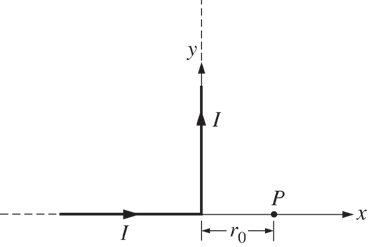
\includegraphics[scale=0.5]{images/img-006-016.png}
\end{center}

% Multiple Choice Question 18
\begin{questions}\setcounter{question}{17}\question
Suppose that the magnetic field due to a very long straight wire carrying current $I$ has magnitude $B_{0}$ at a distance $r_{0}$ from the wire. If the wire is bent into a right angle and placed on the $x y$-axes as shown above, the magnitude of the magnetic field at point $P$ on the $x$-axis at a distance of $r_{0}$ from the bend is most nearly

\begin{oneparchoices}
\choice Zero
\choice $B_{0} / 4$
\choice $B_{0} / 2$
\choice $B_{0}$
\choice $2 B_{0}$
\end{oneparchoices}\end{questions}

